\documentclass[11pt,a4paper]{article}

% ── FONTS ────────────────────────────────────────────────────
\usepackage{fontspec}
\setmainfont{Calibri}
\setsansfont{Calibri}
\newfontfamily{\hindifont}{Nirmala UI}[Script=Devanagari]
\newcommand{\hindi}[1]{{\hindifont #1}}

% ── LAYOUT ───────────────────────────────────────────────────
\usepackage[top=2cm,bottom=2.5cm,left=2.2cm,right=2.2cm]{geometry}
\usepackage{graphicx}
\usepackage{xcolor}
\usepackage{tikz}
\usetikzlibrary{calc,shapes.geometric,arrows.meta,positioning,fit,backgrounds}
\usepackage{tcolorbox}
\tcbuselibrary{skins,breakable}
\usepackage{colortbl}
\usepackage{booktabs}
\usepackage{tabularx}
\usepackage{enumitem}
\usepackage{setspace}
\usepackage{fancyhdr}
\usepackage{titlesec}
\usepackage{hanging}
\usepackage{multicol}
\usepackage{hyperref}
\usepackage{microtype}
\usepackage{array}
\usepackage{caption}

\hypersetup{colorlinks=false,hidelinks}

% ── BRAND COLORS ─────────────────────────────────────────────
\definecolor{navyblue}{HTML}{003566}
\definecolor{gold}{HTML}{C9A84C}
\definecolor{lightgray}{HTML}{F4F6FB}
\definecolor{midgray}{HTML}{D0D6E2}
\definecolor{darkgray}{HTML}{4A4A4A}
\definecolor{accentteal}{HTML}{0077B6}
\definecolor{sectionbg}{HTML}{EEF2FA}
\definecolor{softgreen}{HTML}{E8F5E9}
\definecolor{darkgreen}{HTML}{2E7D32}

% ── SECTION HEADING ──────────────────────────────────────────
\newcommand{\navysectionbox}[1]{%
  \hspace{-2.2cm}%
  \colorbox{navyblue}{%
    \hspace{2.2cm}%
    \parbox[c][0.65cm]{\dimexpr\textwidth+2.0cm}{%
      {\fontsize{12}{14}\selectfont\color{white}\strut\textbf{#1}}%
    }%
  }%
}

\titleformat{\section}[block]{\normalfont}{}{0em}{\navysectionbox}
\titlespacing*{\section}{-2.2cm}{16pt}{8pt}

\titleformat{\subsection}[block]
  {\normalfont\bfseries\fontsize{10.5}{13}\selectfont\color{navyblue}}
  {}{0em}{}
\titlespacing*{\subsection}{0pt}{10pt}{2pt}

% ── HEADER / FOOTER ──────────────────────────────────────────
\setlength{\headheight}{20pt}
\pagestyle{fancy}
\fancyhf{}
\fancyhead[L]{\footnotesize\color{navyblue}\textbf{AIGGPA Bhopal}
  \quad\textbar\quad IT Utilisation Assessment}
\fancyhead[R]{\footnotesize\color{navyblue}April 2026}
\fancyfoot[C]{\footnotesize\color{navyblue}\thepage}
\renewcommand{\headrulewidth}{0.4pt}
\renewcommand{\headrule}{\color{navyblue}\hrule width\headwidth height\headrulewidth}
\renewcommand{\footrulewidth}{1.5pt}
\renewcommand{\footrule}{\color{gold}\hrule width\headwidth height 1.5pt}

% ── CUSTOM BOXES ─────────────────────────────────────────────
\newtcolorbox{goldbox}{
  colback=gold!10, colframe=gold, boxrule=0.7pt, arc=3mm,
  left=10pt,right=10pt,top=8pt,bottom=8pt,breakable}

\newtcolorbox{navybox}{
  colback=sectionbg,colframe=navyblue,boxrule=0.6pt,arc=3mm,
  left=10pt,right=10pt,top=8pt,bottom=8pt,breakable}

\newtcolorbox{greenbox}{
  colback=softgreen,colframe=darkgreen,boxrule=0.6pt,arc=3mm,
  left=10pt,right=10pt,top=8pt,bottom=8pt,breakable}

\newtcolorbox{streamboxa}{
  colback=lightgray,colframe=accentteal,boxrule=1.2pt,arc=3mm,
  lefttitle=8pt,toptitle=4pt,bottomtitle=4pt,
  left=8pt,right=8pt,top=6pt,bottom=6pt,
  title={\bfseries\fontsize{9}{11}\selectfont\color{white}
    Stream A \textbullet{} Department Officials},
  colbacktitle=accentteal,breakable}

\newtcolorbox{streamboxb}{
  colback=lightgray,colframe=navyblue,boxrule=1.2pt,arc=3mm,
  lefttitle=8pt,toptitle=4pt,bottomtitle=4pt,
  left=8pt,right=8pt,top=6pt,bottom=6pt,
  title={\bfseries\fontsize{9}{11}\selectfont\color{white}
    Stream B \textbullet{} IT Department},
  colbacktitle=navyblue,breakable}

% ── LISTS ────────────────────────────────────────────────────
\setlist[itemize]{leftmargin=1.2em,itemsep=2pt,topsep=3pt}
\setlist[enumerate]{leftmargin=1.4em,itemsep=2pt,topsep=3pt}

% ─────────────────────────────────────────────────────────────
\begin{document}
\onehalfspacing

% ═════════════════════════════════════════════════════════════
%  COVER PAGE
% ═════════════════════════════════════════════════════════════
\thispagestyle{empty}
\begin{tikzpicture}[remember picture,overlay]
  \fill[navyblue] (current page.south west) rectangle (current page.north east);
  \fill[gold] (current page.south west)
    rectangle ($(current page.south east)+(0,1.1cm)$);
  \fill[white] ($(current page.south west)+(0,1.1cm)$)
    rectangle ($(current page.south east)+(0,11.8cm)$);
  \fill[accentteal!80]
    ($(current page.south west)+(0,11.8cm)$) --
    ($(current page.south east)+(0,11.8cm)$) --
    ($(current page.south east)+(0,13.2cm)$) --
    ($(current page.south west)+(0,12.4cm)$) -- cycle;
\end{tikzpicture}

\vspace*{6cm}
\begin{center}
  \fontsize{8.5}{10}\selectfont\color{gold!80}
  \textbf{\MakeUppercase{Institutional Research Proposal}}\\[0.7em]
  \fontsize{26}{31}\selectfont\bfseries\color{white}
  Assessment of IT Tool\\[0.15em]
  Utilisation Among\\[0.15em]
  Government Officials\\[0.9em]
  \fontsize{11}{14}\selectfont\color{midgray}
  \hindi{सरकारी अधिकारियों द्वारा आईटी उपकरणों के उपयोग का आकलन}
\end{center}

\vspace*{2.5cm}

\begin{tikzpicture}[remember picture,overlay]
  \node[anchor=south west] at ($(current page.south west)+(2.2cm,1.5cm)$){%
    \begin{minipage}{14cm}
      \footnotesize\color{darkgray}
      \begin{tabular}{@{}ll@{}}
        \textbf{Investigator:} & Aryan Kori \\[3pt]
        \textbf{Institution:}  & AIGGPA, Bhopal \\[3pt]
        \textbf{Departments:}  & School Education \textbullet{} Health
                                 \textbullet{} Forest, Govt.\ of MP \\[3pt]
        \textbf{Date:}         & April 2026 \\
      \end{tabular}
    \end{minipage}%
  };
\end{tikzpicture}

\newpage



% ═════════════════════════════════════════════════════════════
%  BACKGROUND
% ═════════════════════════════════════════════════════════════
\section{Background}

\vspace{0.2cm}
The Government of Madhya Pradesh, architected primarily by technical agencies such as MAP-IT and NIC, has built an impressive portfolio of digital platforms across its key departments:

\begin{itemize}[leftmargin=1.4em]
  \item \textbf{School Education:} Education Portal 3.0 is designed to manage
    approximately 350,000 permanent teachers across 92,000+ schools, covering
    transfers, promotions, attendance, and academic monitoring.\footnote{Government
    of Madhya Pradesh, School Education Department (2025). \textit{Education Portal
    3.0}. \url{https://sederp.educationportal3.in}.}
    Despite its scale and scope, ground-level adoption among district and block
    officials remains uneven.

  \item \textbf{Health:} The department operates HRMIS for HR management, NHM CHETNA
    for frontline health worker training, and has recently launched an AI chatbot called
    ``Ayushman Sakhi'' to help citizens locate hospitals and access health
    information.

  \item \textbf{Forest:} The Forest Department uses satellite data
    to generate real-time encroachment alerts. All wildlife tourism permitting is
    processed through MPOnline.
\end{itemize}

Despite the sophistication of these platforms, institutional observation
reveals that day-to-day workflows at the district and block level still run
on physical registers, courier dak, and informal digital tools. The lack of 
institutionalised usage norms and inadequate front-line computing training are common 
barriers to IT tools in public administration (Bhatnagar, 2004). Often, failures in IT 
adoption originate from a \textit{design-reality gap}: the mismatch between assumptions 
built into a digital system and the actual context in which intended users operate (Heeks, 2003). 

AIGGPA's own training programme feedback consistently surfaces the
same concern: officials know that digital platforms exist, but default to informal
alternatives. A systematic, evidence-based mapping of which tools are being under-used
and why has not yet been conducted for this state.

% ═════════════════════════════════════════════════════════════
%  RATIONALE
% ═════════════════════════════════════════════════════════════
\section{Rationale}

\vspace{0.2cm}

Maximizing the adoption of IT tools translates directly to massive productivity gains 
and structural resilience. The digitization of legacy systems in the public sector is 
widely recognized as a critical strategy for enhancing operational efficiency. 
Current public sector agencies globally face significant hurdles due to aging infrastructure, 
with up to 80\% of IT budgets consumed by "operations and maintenance" of legacy systems, 
starving modern digital transformation efforts (GAO, 2019; Cordella \& Bonina, 2012). 
True modernization bridges the talent and productivity drain by automating manual 
workarounds that are historically rigid in routine document processing.

Rather than relying on disjointed paper ledgers and fragmented records, transitioning 
to cohesive digital platforms allows for centralized, data-driven policy decisions 
at the state level. This proposal aims to study the adoption chokepoints preventing 
Madhya Pradesh's foundational IT platforms from achieving these strategic ROI milestones.

% ═════════════════════════════════════════════════════════════
%  CAPACITY BUILDING
% ═════════════════════════════════════════════════════════════
\section{Capacity Building Framework}

\vspace{0.2cm}

Mission Karmayogi (NPCSCB) has fundamentally transformed the approach to government training,
shifting from a rule-based to a role-based competency framework. The Department of 
Personnel and Training (DoPT) mandates capacity building through the iGOT Karmayogi 
platform, requiring employees to complete digital and functional courses mapped 
to their specific roles.

AIGGPA is Madhya Pradesh's apex institution for civil service training. This research 
will directly fuel AIGGPA's mandate to design evidence-based capacity-building 
programmes. The findings will be used to develop targeted, functional IT modules 
for the iGOT platform, enhancing digital skills and modernising Madhya Pradesh's 
administrative framework in alignment with DoPT guidelines.

% ═════════════════════════════════════════════════════════════
%  THEORETICAL FRAMEWORK
% ═════════════════════════════════════════════════════════════
\section{Theoretical Framework}

\vspace{0.2cm}

To securely bridge individual psychological constraints with the rigid bureaucratic 
realities of state departments, this study employs Venkatesh et al.'s (2003) 
Unified Theory of Acceptance and Use of Technology (UTAUT). UTAUT is the most 
robust framework for evaluating government IT adoption because it explicitly maps 
Organizational Behavior (OB) dynamics alongside individual metrics. The model 
identifies four primary determinants:

\begin{itemize}
  \item \textbf{Performance Expectancy (PE):} the belief that using the system 
    will enhance job performance.
  \item \textbf{Effort Expectancy (EE):} the degree of ease associated with 
    the system's interface.
  \item \textbf{Social Influence (SI):} the degree to which an individual 
    perceives that important others (e.g., District Education Officers, peers) 
    mandate or desire the use of the new system.
  \item \textbf{Facilitating Conditions (FC):} the belief that an organizational 
    and technical infrastructure (e.g., hardware availability, training) exists 
    to support the system.
\end{itemize}

UTAUT resolves a critical flaw in purely psychological models by acknowledging 
hierarchical compliance; if a senior officer mandates a physical wet signature, a 
subordinate's perception of ease-of-use becomes irrelevant. Every data point 
collected will be coded against these four dimensions directly informing AIGGPA 
training designs.

\vspace{0.5cm}

% Visual: UTAUT gap flow diagram
\begin{center}
\begin{tikzpicture}[
  node distance=0.8cm and 1.5cm,
  box/.style={rectangle,rounded corners=3pt,minimum width=2.8cm,
    minimum height=0.6cm,align=center,font=\small\bfseries,
    draw,thick},
  arrow/.style={-{Stealth[length=5pt]},thick,color=navyblue}
]
  \node[box,fill=accentteal!30,draw=accentteal] (pe) {Performance (PE/EE)};
  \node[box,fill=navyblue,text=white,left=of pe] (input) {Official};
  \node[box,fill=gold!40,draw=gold!80!black,below=of pe] (si) {Social Infl.\ (SI)};
  \node[box,fill=gold!40,draw=gold!80!black,below=of si] (fc) {Conditions (FC)};
  \node[box,fill=darkgreen!80,text=white,right=of si] (out) {AIGGPA\\iGOT Module};

  \draw[arrow] (input) |- (pe);
  \draw[arrow] (input) -- (si);
  \draw[arrow] (input) |- (fc);
  \draw[arrow] (pe) -| (out);
  \draw[arrow] (si) -- (out);
  \draw[arrow] (fc) -| (out);
\end{tikzpicture}
\end{center}

\vspace{0.2cm}
\begin{center}
\small\textit{Figure 1. UTAUT classification flow: bureaucratic and individual 
barriers are coded and mapped to a targeted AIGGPA intervention.}
\end{center}

% ═════════════════════════════════════════════════════════════
%  RESEARCH OBJECTIVES
% ═════════════════════════════════════════════════════════════
\section{Research Objectives}

\vspace{0.2cm}
\begin{navybox}
\begin{enumerate}[label={\color{gold}\bfseries\arabic*.},itemsep=5pt]
  \item \textbf{Map actual tool usage} across official categories (identify which
    portals, apps, and informal tools like WhatsApp or Excel each
    class of official uses on a typical working day).
  \item \textbf{Assess document workflow} to understand how officials draft official
    correspondence, process incoming dak, and maintain records.
  \item \textbf{Capture the IT department's perspective} by obtaining usage data,
    system login statistics, and the IT cell's own analysis of low adoption.
  \item \textbf{Classify every barrier} using the UTAUT framework (PE, 
    EE, SI, and FC).
  \item \textbf{Produce actionable recommendations} for AIGGPA training design,
    prioritised by gap severity and departmental need.
\end{enumerate}
\end{navybox}

% ═════════════════════════════════════════════════════════════
%  SCOPE
% ═════════════════════════════════════════════════════════════
\section{Scope}

\vspace{0.2cm}
\renewcommand{\arraystretch}{1.45}
\begin{tabularx}{\textwidth}{%
  >{\columncolor{navyblue}\color{white}\bfseries\small}p{3.2cm}%
  >{\columncolor{lightgray}\small}X}
Departments &
  School Education \textbullet{} Health \textbullet{} Forest
  (Government of Madhya Pradesh) \\
\rowcolor{white}
Respondents &
  Department officials (Class I, II \& III cadres) and IT cell / IT department staff \\
\rowcolor{lightgray}
Office Level &
  State-level Secretariat offices in Bhopal; selected district \& sub-district territorial offices (e.g., Beat Guards, Block Health Officers) \\
\rowcolor{white}
Duration &
  April to June 2026 (approximately 10 weeks) \\
\rowcolor{lightgray}
Exclusions &
  Private contractors; citizen-facing front-end users \\
\rowcolor{white}
Output &
  Gap analysis report and a set of prioritised recommendations for AIGGPA \\
\end{tabularx}

% ═════════════════════════════════════════════════════════════
%  METHODOLOGY
% ═════════════════════════════════════════════════════════════
\section{Methodology}

\vspace{0.2cm}

This study uses a \textbf{mixed-methods, descriptive design}. Quantitative data
(usage frequency, login counts, tool inventories) will be supplemented with
qualitative interview data to explain \textit{why} usage patterns are what they are.
Data collection runs through two parallel streams:

\vspace{0.3cm}
\begin{multicols}{2}
\begin{streamboxa}
\small
\begin{itemize}[leftmargin=1em,itemsep=3pt,topsep=2pt]
  \item What tasks do you perform every day?
  \item Which apps, websites, or tools do you use for them?
  \item Do you use the official departmental portal? If not, why?
  \item Who trained you to use your current tools?
  \item What would make you switch to the official platform?
\end{itemize}
\end{streamboxa}

\columnbreak

\begin{streamboxb}
\small
\begin{itemize}[leftmargin=1em,itemsep=3pt,topsep=2pt]
  \item What platforms have you built and deployed for staff?
  \item \textbf{[Usage Statistics]:} Request aggregated, anonymized portal usage statistics from the departmental IT nodal officer.
  \item How is technical support currently structured?
  \item Have you conducted any usage training? With what outcome?
\end{itemize}
\end{streamboxb}
\end{multicols}

\vspace{0.4cm}

\subsection{Sampling Strategy}

The study will use \textbf{purposive sampling} to ensure representation across
office levels, cadre classes, and departments. Target sample sizes are:

\vspace{0.2cm}
\renewcommand{\arraystretch}{1.4}
\begin{tabularx}{\textwidth}{
  >{\columncolor{navyblue}\color{white}\bfseries\small}p{3.5cm}
  >{\columncolor{lightgray}\centering\arraybackslash\small}p{2cm}
  >{\columncolor{sectionbg}\centering\arraybackslash\small}p{2cm}
  >{\columncolor{lightgray}\centering\arraybackslash\small}p{2cm}
  >{\columncolor{gold!20}\centering\arraybackslash\bfseries\small}X}
\rowcolor{white} System Role Profile & School Edu. & Health & Forest & Total \\
\rowcolor{white} Approvers (Class I/II) & 4 & 4 & 4 & \textbf{12} \\
\rowcolor{lightgray} Data Creators (Class III) & 5 & 5 & 5 & \textbf{15} \\
\rowcolor{white} Field App Users (Territorial) & 6 & 6 & 6 & \textbf{18} \\
\rowcolor{lightgray} IT Nodal Support Staff & 3 & 3 & 3 & \textbf{9} \\
\rowcolor{sectionbg} \textbf{Subtotal} & \textbf{18} & \textbf{18} & \textbf{18} & \textbf{54} \\
\end{tabularx}

\vspace{0.3cm}
Rather than attempting broad statistical representation, a sample of \textbf{54 respondents} 
will be analysed strictly as a series of \textbf{stratified case studies}. This mitigates dataset 
dilution across the four operational tiers while preserving deep qualitative saturation.

\subsection{Data Collection Instruments}

Three instruments will be used:

\begin{enumerate}
  \item \textbf{Semi-structured interview guide (Stream A)}: A 12-question guide
    covering daily tasks, tools in use, perceived barriers, and training history.
    Interviews will run approximately 25--35 minutes and will be conducted in
    Hindi or English per respondent preference.

  \item \textbf{Aggregated Usage Statistics (Stream B)}: A formal request to the 
    IT nodal officer for aggregated, anonymized login metadata and support ticket frequency. 
    \textit{Fallback:} If backend access is denied due to administrative constraints, the 
    study relies exclusively on self-reported usage triangulated via the IT Ecosystem Audit.

  \item \textbf{Direct workflow observation checklist}: A structured observation
    sheet used during brief desk visits to record the actual hardware, open
    applications, and physical materials visible on an official's workstation.
    Observation is non-intrusive and does not require the official to change
    their routine.
\end{enumerate}

\subsection{Data Analysis Plan}

All interview audio (where consent is given) and written field notes will be
\textbf{transcribed verbatim}. Given that government officials frequently 
code-mix Hindi and English during conversation, automated NLP pipelines are highly 
vulnerable to overfitting on this sample size. Therefore, this study relies 
exclusively on a rigorous qualitative \textbf{manual thematic coding pipeline} using 
ATLAS.ti to maximise interpretive depth.

\medskip
\noindent\textbf{Stage 1: Primary Thematic Coding (ATLAS.ti).}
Transcripts will be imported into ATLAS.ti. A \textit{UTAUT thematic codebook} will
be constructed \textit{a priori} for each of the four determinants. For example,
terms such as \textit{``DEO demands paper,''} or \textit{``CM Helpline pressure''}
map to Social Influence (SI); \textit{``no computers working''} maps to Facilitating 
Conditions (FC). The researcher will manually flag transcript sentences and map them 
to these primary UTAUT nodes.

\medskip
\noindent\textbf{Stage 2: Validation and Synthesis.}
Primary tags are reviewed against full transcript context using the thematic
analysis framework of Braun and Clarke (2006) to identify higher-order themes 
(e.g., political reluctance, genuine technical barriers, and \textbf{Informal Process Incentives} 
like slowing file routing for power leverage). To ensure
coding reliability, \textbf{Cohen's kappa} will be calculated on a 10\% randomly
selected sub-sample reviewed independently by a second coder; a target $\kappa \geq
0.70$ is required before the full dataset is finalised.

\medskip
\noindent\textbf{Data Triangulation and Synthesis.}
Numerical usage metrics effectively pressure-test qualitative claims. If qualitative 
coding indicates high Facilitating Conditions (FC) but nodal statistics reveal zero 
logins at a specific block, this discrepancy isolates hidden informal blockers.

To prevent conflating vastly different technological ecosystems, findings are bifurcated into \textbf{Two UTAUT Gap Analysis Matrices}:

\vspace{0.2cm}
\noindent\small\textbf{Matrix A (Secretariat Tools; e.g., e-Office)} \\
\vspace{-0.2cm}
\renewcommand{\arraystretch}{1.4}
\begin{tabularx}{\textwidth}{
  >{\columncolor{navyblue}\color{white}\bfseries\small}p{2.6cm}
  >{\columncolor{lightgray}\centering\arraybackslash\small}X
  >{\columncolor{sectionbg}\centering\arraybackslash\small}X
  >{\columncolor{lightgray}\centering\arraybackslash\small}X
  >{\columncolor{sectionbg}\centering\arraybackslash\small}X}
Department & Perform.\ (PE) & Effort (EE) & Social (SI) & Cond.\ (FC) \\
\rowcolor{white}
School Edu. & & & & \\
\rowcolor{lightgray}
Health & & & & \\
\rowcolor{white}
Forest & & & & \\
\end{tabularx}

\vspace{0.3cm}
\noindent\small\textbf{Matrix B (Field Execution Portals; e.g., Education P3)} \\
\vspace{-0.2cm}
\renewcommand{\arraystretch}{1.4}
\begin{tabularx}{\textwidth}{
  >{\columncolor{accentteal}\color{white}\bfseries\small}p{2.6cm}
  >{\columncolor{lightgray}\centering\arraybackslash\small}X
  >{\columncolor{sectionbg}\centering\arraybackslash\small}X
  >{\columncolor{lightgray}\centering\arraybackslash\small}X
  >{\columncolor{sectionbg}\centering\arraybackslash\small}X}
Department & Perform.\ (PE) & Effort (EE) & Social (SI) & Cond.\ (FC) \\
\rowcolor{white}
School Edu. & & & & \\
\rowcolor{lightgray}
Health & & & & \\
\rowcolor{white}
Forest & & & & \\
\end{tabularx}
\vspace{0.1cm}
\begin{center}
\small\textit{Each cell receives a severity trace (High/Med/Low) derived from ATLAS.ti codes.}
\end{center}

% ═════════════════════════════════════════════════════════════
%  WORK PLAN
% ═════════════════════════════════════════════════════════════
\section{Work Plan}

\vspace{0.2cm}

\renewcommand{\arraystretch}{1.5}
\begin{tabularx}{\textwidth}{
  >{\columncolor{navyblue}\color{white}\bfseries\small\centering}p{1.8cm}
  >{\columncolor{lightgray}\bfseries\small}p{3.2cm}
  >{\columncolor{sectionbg}\small}X}
Phase & Activity & Deliverable / Milestone \\
\rowcolor{white}
Week 1--2 &
  Literature review; finalise theoretical framework &
  Completed proposal; supervisor sign-off \\
\rowcolor{lightgray}
Week 3 &
  Design and pilot-test interview guides and observation checklist &
  Revised instruments approved \\
\rowcolor{white}
Week 4--5 &
  School Education Department: interviews \& observations (Bhopal + 1 district) &
  18 Stratified Case Studies \\
\rowcolor{lightgray}
Week 6--7 &
  Health Department: interviews \& observations &
  18 Stratified Case Studies \\
\rowcolor{white}
Week 8 &
  Forest Department: interviews \& observations &
  18 Stratified Case Studies \\
\rowcolor{lightgray}
Week 9 &
  Data coding, UTAUT classification, gap matrix construction &
  Draft gap analysis matrix \\
\rowcolor{white}
Week 10 &
  Write final report; prepare AIGGPA recommendations deck &
  Final report + presentation \\
\end{tabularx}

% ═════════════════════════════════════════════════════════════
%  LIMITATIONS AND ETHICAL CONSIDERATIONS
% ═════════════════════════════════════════════════════════════
% ═════════════════════════════════════════════════════════════
%  BUDGET ESTIMATE
% ═════════════════════════════════════════════════════════════
\section{Budget Estimate}

\vspace{0.2cm}
This section provides a realistic financial estimate for the qualitative field research study at AIGGPA, covering commercial software licensing, rigorous 10-week transit, and field incidentals for a 54-respondent sample.

\vspace{0.2cm}
\renewcommand{\arraystretch}{1.4}
\begin{tabularx}{\textwidth}{X >{\raggedleft\arraybackslash}p{4cm} r}
\toprule
\textbf{Item Description} & \textbf{Basis of Calculation} & \textbf{Total (INR)} \\
\midrule
Local \& Intercity Transit & Bhopal city auto-rickshaws \& train fare for 1 district & 15,000 \\
Software Licensing & ATLAS.ti Academic / Student License (Annual) & 8,000 \\
Field Surveys Incidentals & Refreshments and access during shadow sessions & 4,500 \\
Consumables \& Printing & Interview guides, stationery, and formal report binding & 2,500 \\
\midrule
\textbf{Total Research Budget} & & \textbf{30,000} \\
\bottomrule
\end{tabularx}
\vspace{0.1cm}
\small\textit{Sources: AIGGPA Institutional Guidelines (2024); Current Madhya Pradesh Transit Rates.}

\vspace{0.1cm}
\small\textit{*Note: Budget represents worst-case out-of-pocket scaling. If AIGGPA holds an existing institutional site-license for NVivo/ATLAS.ti software on network terminals, the 8,000 INR software allocation drops to zero, yielding a revised net ceiling of \textbf{22,000 INR}.}

\section{Limitations and Ethical Considerations}

\vspace{0.2cm}

\subsection{Limitations}

\begin{itemize}
  \item \textbf{Access constraints:} Senior officers (Class I) may have limited
    availability. The study will mitigate this by scheduling interviews flexibly
    and using the observation checklist as a fallback where interviews are declined.
  \item \textbf{Self-reporting bias:} Officials may over-report use of official
    platforms to appear compliant. The observation checklist provides an independent
    check on self-reported data.
  \item \textbf{Hawthorne effect \& OpSec:} Observations may alter behaviour or risk exposure 
    to confidential memos. Rather than intrusive shadowing, we formalise an \textbf{IT Ecosystem Audit}. 
    Observations are strictly limited to the physical IT ecosystem (PC availability, LAN checks, 
    printer connections) and explicitly prevent any viewing of active screen content or secure files.
  \item \textbf{Geographic scope:} Fieldwork is primarily limited to Bhopal state
    offices and one accessible district. Findings may not fully represent rural
    district realities.
  \item \textbf{Generalisability:} Results are contextualised to Madhya Pradesh and
    cannot be directly extrapolated to other states without replication.
\end{itemize}

\subsection{Ethical Considerations}

\begin{itemize}
  \item All participation is \textbf{voluntary}. Respondents will be briefed on the
    purpose of the study before the interview begins.
  \item No personally identifiable information will appear in the final report.
    Designations and departments will be used in place of names.
  \item Interview notes will be stored securely on a password-protected device and
    will not be shared outside the AIGGPA internship supervision structure.
  \item No audio recordings will be made without explicit informed consent.
\end{itemize}

% ═════════════════════════════════════════════════════════════
%  EXPECTED OUTPUT
% ═════════════════════════════════════════════════════════════
\section{Expected Output}

\vspace{0.2cm}
\begin{multicols}{3}

\begin{tcolorbox}[colback=navyblue,colframe=navyblue,arc=4mm,
  left=8pt,right=8pt,top=8pt,bottom=8pt]
\centering
{\color{gold}\bfseries\large 01}\\[4pt]
{\color{white}\small\textbf{IT Utilisation Map}\\[4pt]
Role-wise and level-wise map of tools used vs.\ tools available, per department}
\end{tcolorbox}

\columnbreak

\begin{tcolorbox}[colback=accentteal,colframe=accentteal,arc=4mm,
  left=8pt,right=8pt,top=8pt,bottom=8pt]
\centering
{\color{white}\bfseries\large 02}\\[4pt]
{\color{white}\small\textbf{Bifurcated UTAUT Matrices}\\[4pt]
Separating Policy toolsets from Field execution portals}
\end{tcolorbox}

\columnbreak

\begin{tcolorbox}[colback=gold,colframe=gold,arc=4mm,
  left=8pt,right=8pt,top=8pt,bottom=8pt]
\centering
{\color{navyblue}\bfseries\large 03}\\[4pt]
{\color{navyblue}\small\textbf{AIGGPA Recommendations}\\[4pt]
Targeted capacity-building interventions prioritised by gap severity}
\end{tcolorbox}

\end{multicols}

\vspace{0.4cm}
\begin{greenbox}
\textbf{\color{darkgreen}Bifurcated Impact Pathway:} The gap matrix will explicitly bifurcate outputs to avoid treating technology adoption as purely a training problem:
\begin{enumerate}[label=\textcolor{darkgreen}{\bfseries\arabic*.},itemsep=2pt,leftmargin=1.5em]
  \item \textbf{Training Interventions (PE \& EE Gaps):} Forwarded to the iGOT capacity building division to design specific module upgrades.
  \item \textbf{Policy/Infrastructure Briefs (SI \& FC Gaps):} Forwarded to Department Secretaries as actionable memos (e.g., funding hardware repairs, or officially banning paper submittals) to resolve structural blockers that cannot be trained away.
\end{enumerate}
\end{greenbox}

% ═════════════════════════════════════════════════════════════
%  REFERENCES
% ═════════════════════════════════════════════════════════════
\section{References}

\vspace{0.2cm}
\small\setlength{\parindent}{0pt}\singlespacing
\begin{hangparas}{1.27cm}{1}

Alrawabdeh, W. (2014). Examining factors affecting digital platform adoption in Jordan.
\textit{International Journal of Business and Social Science}, \textit{5}(8), 232--241.

\vspace{4pt}
Atal Bihari Vajpayee Institute of Good Governance and Policy Analysis (AIGGPA). (2024). \textit{Institutional Research Guidelines}. Government of Madhya Pradesh.

\vspace{4pt}
Bhatnagar, S. (2004). \textit{IT platforms: From vision to implementation: A
practical guide with case studies}. Sage Publications.

\vspace{4pt}
Braun, V., \& Clarke, V. (2006). Using thematic analysis in psychology.
\textit{Qualitative Research in Psychology}, \textit{3}(2), 77--101.

\vspace{4pt}
Cordella, A., \& Bonina, C. M. (2012). A public value perspective for ICT enabled public sector reforms: A theoretical reflection. \textit{Government Information Quarterly}, \textit{29}(4), 512--520.

\vspace{4pt}
Government of India, Department of Personnel \& Training. (2020).
\textit{National programme for civil services capacity building (Mission Karmayogi)}.
Ministry of Personnel, Public Grievances and Pensions.

\vspace{4pt}
Government of India, Ministry of Finance (2026). \textit{Union Budget 2026-27: Expenditure Profile}.
Economic Division, Department of Economic Affairs.

\vspace{4pt}
Government of Madhya Pradesh, School Education Department. (2025).
\textit{Education Portal 3.0}. \url{https://sederp.educationportal3.in}

\vspace{4pt}
Government of Madhya Pradesh, Forest Department. (2024).
\textit{AI-based real-time forest alert system}.
\url{https://forest.mponline.gov.in/}

\vspace{4pt}
Heeks, R. (2003). \textit{Most IT-for-development projects fail: How can
risks be reduced?} (iGovernment Working Paper No. 14).
Institute for Development Policy and Management, University of Manchester.

\vspace{4pt}
Ministry of Electronics \& Information Technology, Government of India. (2015).
\textit{Digital India: Programme to transform India into a digitally empowered society
and knowledge economy}. \url{https://digitalindia.gov.in/}

\vspace{4pt}
National Health Mission, Madhya Pradesh. (2024).
\textit{NHM CHETNA portal}. \url{https://ntep.in/}

\vspace{4pt}
United States Government Accountability Office (GAO). (2019). \textit{Information Technology: Agencies Need to Develop Modernization Plans for Critical Legacy Systems} (GAO-19-471).

\vspace{4pt}
Venkatesh, V., Morris, M. G., Davis, G. B., \& Davis, F. D. (2003). User acceptance of information technology: Toward a unified view. \textit{MIS Quarterly}, 425--478.

\end{hangparas}

\end{document}
